\documentclass[conference, a4paper]{IEEEtran}
\IEEEoverridecommandlockouts
\usepackage[turkish]{babel}
\usepackage[utf8]{inputenc}
\usepackage[T1]{fontenc}
\usepackage[pdftex]{graphicx}
\usepackage{multirow}
\usepackage{cite}
\usepackage[cmex10]{amsmath}
\usepackage{siunitx}
\usepackage{array}
\usepackage[caption=false,lofdepth,lotdepth]{subfig}
\usepackage{booktabs}
\usepackage{float}
\usepackage{url}
\usepackage{acronym}

\setlength{\textfloatsep}{5pt}

\AtBeginDocument{%
	\renewcommand\tablename{TABLO}
}

\AtBeginDocument{%
	\renewcommand\abstractname{Abstract}
}

\graphicspath{{../results/}{../results/plots/}}

\begin{document}
\shorthandoff{=}

\title{NPM Tedarik Zincirinde Topolojik Risk Analizi ve Kritiklik Haritalaması\\
 Topological Risk Analysis and Criticality Mapping in the NPM Supply Chain}

\author{\IEEEauthorblockN{Yusuf Talha ARABACI}
\IEEEauthorblockA{\textit{Yazılım Mühendisliği Anabilim Dalı} \\
\textit{Karabük Üniversitesi}\\
Karabük, Türkiye \\
yusuftalhaarabaci@hotmail.com}
}

\maketitle

\begin{ozet}
Modern yazılım geliştirmenin omurgasını oluşturan NPM ekosistemi, tekil bir bağımlılıktaki güvenlik zafiyetinin veya kötü niyetli kod değişikliğinin, dolaylı bağlantılar üzerinden hızla yayılarak sistemik bir krize dönüşme potansiyelini taşır. Bu araştırma, paketlerin kod içeriğine odaklanan geleneksel yaklaşımların ötesine geçerek, paketler arası ilişkilerin \emph{topolojik} izlerini sürer ve ekosistemin en kritik düğümlerini bu yapısal analizle saptar. Çalışmada, en fazla bağımlıya sahip 1000 paket üzerinden 7 kademe derinliğinde yönlü bir bağımlılık ağı inşa edilmiştir. Ağ üzerinde hesaplanan in-degree, out-degree ve betweenness merkeziyet ölçümleri, min-max normalizasyonu ile işlenerek \emph{Bileşik Risk Skoru} (BRS) altında bütünleşik bir metriğe dönüştürülmüştür. Kritik düğümlerin ağdan çıkarılmasının en büyük bağlı bileşen (LCC) ve ağ erişilebilirliği üzerindeki yıkıcı etkisini ölçmek adına sağlamlık ve kaskad analizleri uygulanmıştır. Elde edilen bulgular, ağın iskeletini oluşturan az sayıda paketin sistemik riskin aslan payını yüklendiğini ve bu düğümlerin güvenliğinin tüm ekosistem için hayati bir zorunluluk olduğunu gözler önüne sermektedir.
\end{ozet}

\begin{IEEEanahtar}
Yazılım tedarik zinciri güvenliği, NPM, bağımlılık ağı analizi, topolojik risk, kaskad etkisi.
\end{IEEEanahtar}

\begin{abstract}
In the NPM ecosystem, which lies at the heart of modern software development, a vulnerability or malicious alteration in a single dependency can propagate rapidly through the transitive dependency chain, impacting thousands of projects within a short timeframe. Unlike traditional approaches focusing on code content, this study aims to identify high-impact nodes by analyzing the \emph{topological} patterns of inter-package relationships. A directed dependency graph was constructed using the Top 1000 packages selected based on the highest number of dependents, extending to a depth of 7 levels. In-degree, out-degree, and betweenness centralities calculated on this network were processed via min–max normalization and combined into a unified metric termed the \emph{Composite Risk Score} (BRS). Robustness and cascade analyses were conducted to measure the impact of removing critical nodes on the largest connected component and reachability. The results indicate that a small number of backbone packages carry a significant portion of the systemic risk, highlighting that the security of these nodes is vital for the entire ecosystem.
\end{abstract}

\begin{IEEEkeywords}
Software supply chain security, NPM, dependency network analysis, topological risk, cascade effect.
\end{IEEEkeywords}

\IEEEpeerreviewmaketitle

\section{G{\footnotesize İ}r{\footnotesize İ}ş}
Yazılım geliştirme pratikleri, verimliliği maksimize etmek ve tekerleği yeniden icat etmekten kaçınmak adına NPM, PyPI ve RubyGems gibi açık kaynak paket yöneticilerine giderek daha fazla yaslanmaktadır. Bu modüler mimari, geliştirme süreçlerine ivme kazandırsa da, tedarik zincirindeki en ufak bir çatlağın sistemik bir krize evrilmesine zemin hazırlayan kırılgan bir yapı ortaya çıkarmıştır \cite{lit1}. Milyonlarca paketi ve bunlar arasındaki girift bağımlılık ağını barındıran NPM ekosistemi, sunduğu geniş saldırı yüzeyiyle tehdit aktörleri için cazip bir hedef konumundadır. Literatürdeki bulgular, bu ağın "küçük dünya" (small-world) karakteristiği sergilediğini, dolayısıyla az sayıda bakımcının veya paketin ekosistem üzerinde orantısız bir etki gücüne sahip olduğunu doğrulamaktadır \cite{lit20, lit16, lit25}.

Tedarik zinciri saldırıları, güvenilir paketlerin ele geçirilmesinden isim benzerliği (typosquatting) tuzaklarına kadar geniş bir yelpazede tezahür eder. "Backstabber’s Knife Collection" \cite{lit4} ve "The Hitchhiker’s Guide" \cite{lit24} gibi kapsamlı derlemeler, saldırıların anatomisini kurulum ve çalışma zamanı (runtime) evreleri üzerinden irdelerken; Duan ve ark. \cite{lit28}, kayıt defteri (registry) düzeyindeki istismarlara odaklanarak yüzlerce kötü niyetli paketin varlığını belgelemiştir. Bu tehditlere karşı Amalfi \cite{lit19}, Cerebro ve OSCAR \cite{lit29} gibi makine öğrenmesi ve dinamik analiz tabanlı savunma mekanizmaları geliştirilmiş olsa da, ekosistemin devasa ölçeği, her bir paketin derinlemesine taranmasını maliyet ve zaman açısından sürdürülemez kılmaktadır.

Mevcut literatür kritik düğümlerin varlığını teslim etmekle birlikte, bu düğümlerin sistematik tespiti ve \textit{in-toto} \cite{lit13} gibi güvenlik politikalarına entegrasyonu konusunda metodolojik bir boşluk barındırmaktadır. Analizler ekseriyetle popülerlik (indirme sayısı) veya statik kod analizi gibi metriklere hapsolmakta, ağ topolojisinden neşet eden yapısal riskleri bütüncül bir perspektifle değerlendirmekte yetersiz kalmaktadır. Bu çalışma, paket içeriklerinden soyutlanarak, yalnızca paketler arası bağımlılıkların topolojik mimarisine odaklanmakta ve yapısal riskin haritalandırılması için özgün bir metodoloji sunarak söz konusu boşluğu doldurmayı amaçlamaktadır.

Araştırmanın literatüre sunduğu temel katkılar şunlardır:
\begin{enumerate}
  \item Resmî çözümleme kuralları çerçevesinde inşa edilen yönlü graf üzerinde in-degree, out-degree ve betweenness ölçümleri min–max yöntemiyle ölçeklenmiş; \(w_{in}=0.5\), \(w_{out}=0.2\), \(w_{btw}=0.3\) ağırlıklarıyla sentezlenerek \textbf{Bileşik Risk Skoru (BRS)} tanımlanmıştır.
  \item BRS sıralaması, kaskad etki ve en büyük bağlı bileşen (LCC) analizleriyle ilişkilendirilerek, topolojik riskin sistemik yansımaları nicel verilerle ortaya konulmuştur.
  \item Elde edilen bulgular, güvenlik analistleri ve paket yöneticileri için önceliklendirilmiş bir izleme listesi sunarak, kısıtlı güvenlik kaynaklarının nokta atışı kullanılabilmesine olanak tanımaktadır.
\end{enumerate}

\section{Ver{\footnotesize İ} ve Yöntem}

\subsection{Veri Setinin Oluşturulması ve Kapsam}
NPM ekosisteminin risk haritasını çıkarmak amacıyla yürütülen ön çalışmalarda, "Most Downloaded" ve "Trending" gibi farklı örneklem stratejileri masaya yatırılmıştır. Ancak yapılan fizibilite analizleri, tedarik zinciri riskini en gerçekçi şekilde modelleyen yaklaşımın, en fazla sayıda projeye altyapı sağlayan paketlere odaklanmak olduğunu göstermiştir. Dolayısıyla analizin başlangıç noktası olarak, ekosistemin kılcal damarlarına kadar nüfuz etmiş (örneğin \texttt{lodash}, \texttt{chalk}, \texttt{express}) ilk 1000 paket seçilmiştir. Bu paketler, hiyerarşinin uç noktalarındaki son kullanıcı uygulamalarından ziyade, tüm sistemin üzerine inşa edildiği temel yapı taşlarını temsil eder.

NPM ekosistemi, en üstte uygulamaların yer aldığı ve aşağıya doğru kütüphanelere dallanan ters bir ağaç yapısını andırır; bu çalışmada seçilen örneklem ise sistemin yükünü sırtlayan merkezi katmana tekabül etmektedir. Analiz sürecinde, bu temel paketlerin \texttt{dependencies} listeleri izlenerek 7. dereceye kadar inilmiş ve tedarik zincirinin derinliği haritalandırılmıştır. Paketlerin, kendilerini kullanan üst katman projelerine dair doğrudan bir referans içermemesi, analizi yukarı yönlü (upstream) takip etmeyi güçleştirmektedir. Bu teknik kısıtlılığı aşmak adına, NPM API aracılığıyla her paketin toplam "bağımlı sayısı" (dependents) sorgulanmış ve bu metrik, örneklem seçiminde ana kriter olarak belirlenerek analizin ekosistemin en kritik katmanına odaklanması sağlanmıştır.

Yalnızca üretim bağımlılıkları (\texttt{dependencies}) filtreye tabi tutulmuş ve döngüsel referanslar ayıklanarak 1.506 düğüm ve 3.058 kenardan müteşekkil yönlü bir graf inşa edilmiştir. Ortaya çıkan bu graf, ekosistemdeki kritik düğümleri ve yapısal kırılganlıkları kristalize etmektedir. Grafik inşası ve analizi Python tabanlı NetworkX kütüphanesiyle gerçekleştirilmiş; veri setleri ve Gephi uyumlu çıktılar (\texttt{gephi\_nodes.csv}, \texttt{gephi\_edges.csv}) \texttt{results/} dizininde arşivlenmiştir.

\subsection{Merkeziyet Ölçüleri ve Normalizasyon}
Ağdaki her bir paketin önemini ve sistemik risk potansiyelini nicel olarak ifade edebilmek adına üç temel merkeziyet metriğine başvurulmuştur:
\begin{itemize}
    \item \textbf{In-Degree:} Bir paketin popülaritesini ve doğrudan etki alanını tanımlayan bu metrik, o pakete doğrudan bağımlı olan diğer paketlerin sayısını ifade eder.
    \item \textbf{Out-Degree:} Bir paketin işlevselliğini sürdürebilmek için ihtiyaç duyduğu dış bağımlılıkların sayısıdır. Yüksek bir out-degree değeri, paketin saldırı yüzeyinin genişliğine ve dış kaynaklı risklere karşı kırılganlığına işaret eder.
    \item \textbf{Betweenness (Arasılık):} Bir paketin, ağdaki diğer düğümler arasındaki en kısa yollar üzerinde ne sıklıkla yer aldığını ölçer. Bu metrik, paketin ağ içindeki "köprü" rolünü ve bilgi/risk akışını denetleme kapasitesini yansıtır. Hesaplama maliyetini optimize etmek amacıyla \(k = 20\) örneklemli bir yaklaşım benimsenmiştir.
\end{itemize}
Farklı ölçeklerdeki bu üç metriği ortak bir paydada buluşturmak için her biri min-max normalizasyonu ile [0,1] aralığına indirgenmiştir:
\[
x' = \frac{x - \min(x)}{\max(x)-\min(x)}
\]

\subsection{Bileşik Risk Skoru (BRS)}
Normalizasyon sürecinden geçen değerler, her bir metriğin risk potansiyelini farklı boyutlarıyla yansıtması gözetilerek, ağırlıklı bir formülle bütünleşik bir skora tahvil edilmiştir:
\[
\text{BRS} = 0.5 \cdot in' + 0.2 \cdot out' + 0.3 \cdot btw'
\]
Bu formülasyonda in-degree'ye en yüksek ağırlığın ($w_{in}=0.5$) atfedilmesi, bir paketin tehlikeye girmesinin doğrudan etkileyeceği proje sayısının sistemik risk açısından taşıdığı kritik öneme dayanır. Ağdaki dolaylı yayılım riskini ve stratejik konumu temsil eden betweenness ise ikinci en yüksek ağırlıkla ($w_{btw}=0.3$) modeldeki yerini almıştır.

\subsection{Sağlamlık ve Kaskad Analizleri}
BRS metriğinin sistemik riski öngörme kapasitesini sınamak amacıyla "hedefli saldırı" simülasyonları kurgulanmıştır. Bu senaryolarda, en yüksek BRS skoruna sahip paketler ağdan kademeli olarak izole edilmiş; bu müdahalenin En Büyük Bağlı Bileşen (LCC) boyutuna, ortalama yol uzunluğuna ve ağın genel erişilebilirliğine (reachability) olan etkisi mercek altına alınmıştır. Buna ek olarak, her bir düğümün potansiyel etki alanını (transitif kapanış) ölçen bir kaskad analizi yürütülerek, BRS'nin öngörü gücü çapraz doğrulamaya tabi tutulmuştur.

\section{Bulgular ve Değerlend{\footnotesize İ}rme}

\subsection{Ağ Topolojisi ve Derece Dağılımı}
\begin{table}[H]
\centering
\caption{\textsc{Ağ İstatistikleri}}
\label{tab:stats}
\begin{tabular}{lc}
\toprule
Metrik & Değer \\
\midrule
Düğüm Sayısı (Nodes) & 1506 \\
Kenar Sayısı (Edges) & 3058 \\
Ortalama Derece (Avg Degree) & 2.03 \\
Yoğunluk (Density) & 0.0013 \\
Ortalama Arasılık (Avg Betweenness) & $1.05 \times 10^{-5}$ \\
\bottomrule
\end{tabular}
\end{table}

\begin{figure}[H]
\centering
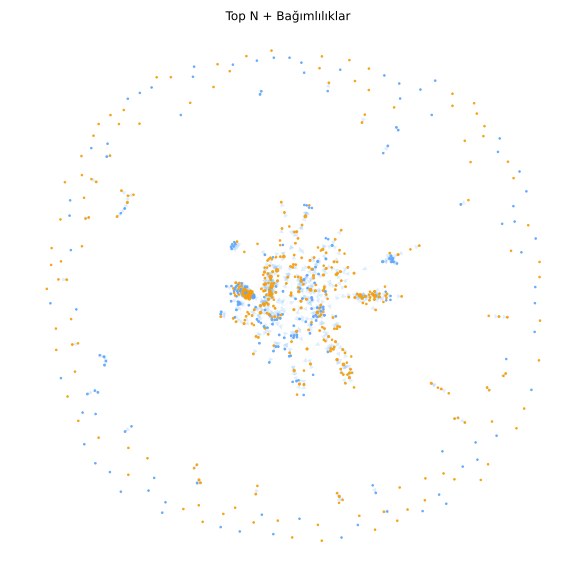
\includegraphics[width=\linewidth]{network_full_topN.png}
\caption{Top 1000 paket ağının görselleştirmesi. Yoğun bölgeler, ekosistemin omurgasını oluşturan alt kümeleri işaret etmektedir.}
\label{fig:network}
\end{figure}

\begin{figure}[H]
\centering
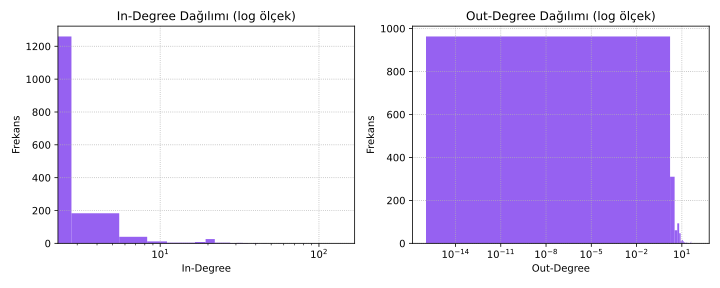
\includegraphics[width=\linewidth]{degree_histograms.png}
\caption{In-degree ve out-degree histogramları. Dağılımın ağır kuyruklu (heavy-tailed) yapısı, merkeziyetin az sayıda pakette toplandığını doğrulamaktadır.}
\label{fig:histograms}
\end{figure}

Şekil \ref{fig:network}'te sunulan ağ görselleştirmesi, yapının homojen bir dağılım yerine belirli odak noktalarında yoğunlaşan belirgin bir kümelenme (clustering) eğilimi taşıdığını göstermektedir. Derece dağılımlarının irdelendiği Şekil \ref{fig:histograms}, bu yapısal karakteristiği daha somut verilerle destekler: Ağ, düğümlerin kahir ekseriyetinin sınırlı sayıda bağlantıya sahip olduğu, buna karşın "hub" niteliğindeki elit bir grubun yüzlerce bağlantıyı yönettiği, "ölçekten bağımsız" (scale-free) bir topoloji arz etmektedir. Dağılımın ağır kuyruklu (heavy-tailed) yapısı, merkeziyetin ve dolayısıyla riskin, az sayıda paketin tekelinde toplandığının açık bir göstergesidir.

\subsection{Merkeziyet İlişkileri}
\begin{figure}[H]
\centering
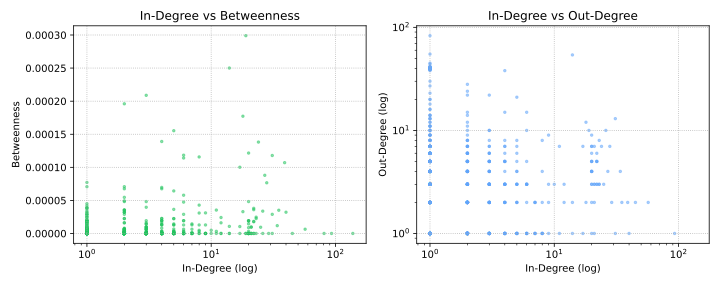
\includegraphics[width=\linewidth]{scatter_correlations.png}
\caption{Merkeziyet ölçüleri arasındaki korelasyonlar.}
\label{fig:scatter}
\end{figure}

Merkeziyet ölçümleri arasındaki korelasyonlar (Şekil \ref{fig:scatter}) mercek altına alındığında, in-degree ile betweenness arasında pozitif yönlü ancak asimetrik bir ilişki göze çarpar. Bu bulgu, yüksek popülerliğe (in-degree) sahip olmayan bazı paketlerin, ağın izole kümelerini birbirine bağlayan kritik köprüler (yüksek betweenness) olarak stratejik bir misyon üstlenebildiğine işaret eder. Dolayısıyla, odağını yalnızca popülerliğe kilitleyen analizler, bu tür "gizli" kritiklikleri ıskalama riskiyle karşı karşıyadır.

\subsection{Kritik Düğümlerin Analizi}
\begin{table}[H]
\centering
\caption{\textsc{Top 10 In-Degree}}
\label{tab:indegree}
\resizebox{\linewidth}{!}{%
\begin{tabular}{lrrrr}
\toprule
Paket & In-Degree & Out-Degree & Betweenness & TopN? \\
\midrule
@babel/helper-plugin-utils & 110 & 0 & 0.000000 & True \\
call-bound & 41 & 2 & 0.000283 & False \\
postcss-value-parser & 39 & 0 & 0.000000 & True \\
call-bind & 36 & 4 & 0.000000 & False \\
@types/node & 34 & 1 & 0.000067 & False \\
debug & 34 & 1 & 0.000100 & True \\
es-errors & 33 & 0 & 0.000000 & False \\
@babel/types & 32 & 2 & 0.000236 & True \\
define-properties & 29 & 3 & 0.000000 & False \\
chalk & 28 & 0 & 0.000000 & False \\
\bottomrule
\end{tabular}%
}
\end{table}

\begin{table}[H]
\centering
\caption{\textsc{Top 10 Out-Degree}}
\label{tab:outdegree}
\resizebox{\linewidth}{!}{%
\begin{tabular}{lrrrr}
\toprule
Paket & Out-Degree & In-Degree & Betweenness & TopN? \\
\midrule
@babel/preset-env & 70 & 3 & 0.000000 & True \\
postcss-preset-env & 67 & 1 & 0.000000 & True \\
es-abstract & 54 & 17 & 0.000000 & False \\
react-scripts & 48 & 0 & 0.000000 & True \\
workbox-build & 37 & 1 & 0.000000 & True \\
eslint & 34 & 1 & 0.000000 & True \\
cssnano-preset-default & 30 & 1 & 0.000000 & True \\
webpack-dev-server & 28 & 1 & 0.000000 & True \\
@jest/core & 28 & 2 & 0.000000 & True \\
express & 27 & 1 & 0.000000 & True \\
\bottomrule
\end{tabular}%
}
\end{table}

\begin{table}[H]
\centering
\caption{\textsc{Top 10 Betweenness}}
\label{tab:betweenness}
\resizebox{\linewidth}{!}{%
\begin{tabular}{lrrrr}
\toprule
Paket & Betweenness & In-Degree & Out-Degree & TopN? \\
\midrule
jest-circus & 0.001144 & 1 & 20 & False \\
@babel/core & 0.001112 & 12 & 15 & True \\
babel-jest & 0.001087 & 2 & 7 & True \\
jest-runner & 0.001000 & 2 & 22 & True \\
@babel/helper-create-class-features-plugin & 0.000798 & 10 & 7 & True \\
get-intrinsic & 0.000771 & 22 & 10 & True \\
jest-snapshot & 0.000549 & 6 & 21 & True \\
@babel/traverse & 0.000523 & 20 & 7 & True \\
babel-preset-current-node-syntax & 0.000499 & 2 & 15 & False \\
babel-plugin-istanbul & 0.000466 & 2 & 5 & True \\
\bottomrule
\end{tabular}%
}
\end{table}
Merkeziyet metriklerine dayalı sıralamalar, ekosistemdeki farklı kritiklik profillerini ayrıştırmamıza olanak tanır. Tablo \ref{tab:indegree}'de listelenen ve in-degree zirvesini tutan paketler, ekosistemin en popüler ve güven duyulan yapı taşlarını temsil eder. Öte yandan, Tablo \ref{tab:outdegree}'de öne çıkan \texttt{@babel/preset-env} gibi paketler, sahip oldukları yoğun dış bağımlılıklar nedeniyle geniş bir saldırı yüzeyi sunmakta ve tedarik zincirinin alt katmanlarından sızabilecek tehditlere karşı kırılgan bir profil çizmektedir. Tablo \ref{tab:betweenness} ise, popülerlikten bağımsız olarak, ağdaki bilgi ve risk trafiğini yöneten \texttt{jest-circus} gibi stratejik darboğazları ifşa eder. Bu üç farklı perspektif, tek boyutlu analizlerin riskin bütüncül resmini çizmekte yetersiz kalacağını kanıtlar niteliktedir.

\subsection{Bileşik Risk Skoru (BRS) Sıralaması}
\begin{figure}[H]
\centering
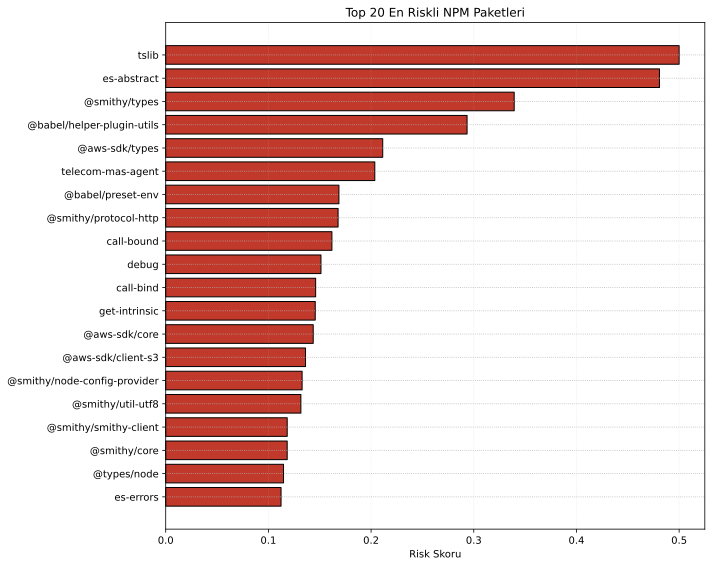
\includegraphics[width=\linewidth]{top20_risk_scores.png}
\caption{En yüksek Bileşik Risk Skoruna (BRS) sahip 20 paket.}
\label{fig:risk_scores}
\end{figure}

\begin{table}[H]
\centering
\caption{\textsc{Top 20 Bileşik Risk Skoru (BRS)}}
\label{tab:risk}
\resizebox{\linewidth}{!}{%
\begin{tabular}{lrrrrr}
\toprule
Paket & Risk & In-Degree & Out-Degree & Betweenness & TopN? \\
\midrule
@babel/helper-plugin-utils & 0.500000 & 110 & 0 & 0.000000 & True \\
@babel/core & 0.388827 & 12 & 15 & 0.001112 & True \\
jest-circus & 0.361688 & 1 & 20 & 0.001144 & False \\
jest-runner & 0.334157 & 2 & 22 & 0.001000 & True \\
get-intrinsic & 0.330606 & 22 & 10 & 0.000771 & True \\
babel-jest & 0.313975 & 2 & 7 & 0.001087 & True \\
@babel/helper-create-class-features-plugin & 0.274757 & 10 & 7 & 0.000798 & True \\
call-bound & 0.266206 & 41 & 2 & 0.000283 & False \\
@babel/traverse & 0.248118 & 20 & 7 & 0.000523 & True \\
es-abstract & 0.231558 & 17 & 54 & 0.000000 & False \\
jest-snapshot & 0.231168 & 6 & 21 & 0.000549 & True \\
@babel/preset-env & 0.213636 & 3 & 70 & 0.000000 & True \\
@babel/types & 0.212942 & 32 & 2 & 0.000236 & True \\
postcss-preset-env & 0.195974 & 1 & 67 & 0.000000 & True \\
@jest/types & 0.193414 & 26 & 7 & 0.000211 & True \\
debug & 0.183565 & 34 & 1 & 0.000100 & True \\
babel-preset-current-node-syntax & 0.182762 & 2 & 15 & 0.000499 & False \\
postcss-value-parser & 0.177273 & 39 & 0 & 0.000000 & True \\
call-bind & 0.175065 & 36 & 4 & 0.000000 & False \\
@types/node & 0.174844 & 34 & 1 & 0.000067 & False \\
\bottomrule
\end{tabular}%
}
\end{table}
Geliştirilen BRS modeli, üç farklı risk boyutunu (popülerlik, bağımlılık yüzeyi, köprü rolü) tek bir potada eriterek, tekil metriklerin yakalayamadığı hibrit risk profillerini görünür kılar. Şekil \ref{fig:risk_scores} ve Tablo \ref{tab:risk}'te izlendiği üzere, \texttt{@babel/core} ve \texttt{jest-runner} gibi paketler, hem yüksek popülariteleri hem de ağdaki stratejik konumları sebebiyle risk sıralamasının zirvesine yerleşmektedir. Bu hiyerarşi, güvenlik denetimleri ve kaynak tahsisinde önceliklendirilmesi elzem olan "yüksek değerli hedefleri" (high-value targets) tartışmaya yer bırakmayacak netlikte tanımlar.

\subsection{Sistemik Etki ve Kaskad Analizi}
\begin{figure}[H]
\centering
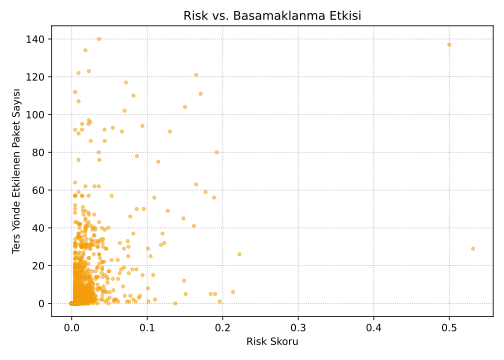
\includegraphics[width=\linewidth]{risk_vs_cascade.png}
\caption{BRS ile kaskad etki (erişilebilirlik) arasındaki ilişki.}
\label{fig:cascade}
\end{figure}

\begin{figure}[H]
\centering
\includegraphics[width=\linewidth]{top20_cascade_impact.png}
\caption{İlk 20 paketin çıkarılmasının LCC ve erişilebilirlik üzerindeki yıkıcı etkisi.}
\label{fig:impact}
\end{figure}
BRS'nin sistemik riski öngörme kabiliyetini sınayan hedefli saldırı simülasyonları, modelin geçerliliğini çarpıcı bir biçimde ortaya koymaktadır. Şekil \ref{fig:impact}'te görüldüğü üzere, BRS zirvesindeki paketlerin ağdan koparılması, rastgele düğüm seçimine kıyasla En Büyük Bağlı Bileşen (LCC) boyutunda çok daha yıkıcı bir çöküşe neden olmakta ve ağın bütünlüğünü hızla parçalamaktadır. BRS skoru ile kaskad etki (bir düğümün kaybından etkilenen toplam paket sayısı) arasındaki güçlü pozitif korelasyon (Şekil \ref{fig:cascade}) da bu tespiti perçinler. Bu veriler, BRS'nin yalnızca statik bir kritiklik ölçütü olmadığını, aynı zamanda bir düğümün ele geçirilmesinin tüm ekosistemde tetikleyebileceği zincirleme reaksiyonun da güvenilir bir habercisi olduğunu teyit etmektedir.

\section{Tartışma ve Sonuç}
Bu araştırma, NPM ekosistemindeki sistemik riski, paket içeriğinden bağımsız olarak salt topolojik parametreler üzerinden modelleyen BRS (Bileşik Risk Skoru) metodolojisini literatüre kazandırmış ve geçerliliğini ampirik olarak kanıtlamıştır. Yürütülen analizler, ekosistem güvenliğinin, tehlikeye girmeleri halinde domino etkisiyle ağın bütünlüğünü çökertme potansiyeli taşıyan az sayıda "omurga" paketin sırtında yükseldiğini nicel verilerle doğrulamıştır.

Elde edilen bulgular ve önerilen model, teorik bir egzersiz olmanın ötesine geçerek, yazılım tedarik zinciri güvenliğini operasyonel düzeyde tahkim edecek somut stratejiler sunmaktadır:
\begin{itemize}
    \item \textbf{Tespit Hatlarında Önceliklendirme:} Amalfi ve Cerebro gibi savunma mekanizmalarında tarama kaynaklarının, BRS skoru yüksek paketlere kanalize edilerek verimliliğin artırılması.
    \item \textbf{Politika Geliştirme:} in-toto gibi katı güvenlik protokollerinin ve dijital imza zorunluluğunun, öncelikle bu çalışmada saptanan kritik düğümlere uygulanarak riskin kaynağında boğulması.
    \item \textbf{Bakımcı Farkındalığı:} Kritik paket sahiplerine risk skorlarının bildirilmesi yoluyla, iki faktörlü kimlik doğrulama (2FA) ve daha titiz kod inceleme pratiklerinin benimsenmesinin teşvik edilmesi.
\end{itemize}

Gelecek çalışmaların rotası, geliştirilen modeli paketler arasındaki teknik bağların ötesine taşıyarak, geliştirici ağları (maintainer networks) ve sosyal bağımlılıklar gibi insan faktörlerini de kapsayacak şekilde genişletmektir. Ayrıca, ekosistemin zamana bağlı dinamiklerini mercek altına alan boylamsal (temporal) bir yaklaşım, riskin evrimini ve dönüşümünü anlamlandırmak adına paha biçilmez bir perspektif sunacaktır.

\section{Yen{\footnotesize İ}den Üret{\footnotesize İ}leb{\footnotesize İ}rl{\footnotesize İ}k}
Çalışmanın şeffaflığını ve tekrarlanabilirliğini sağlamak adına tüm kaynak kodlar ve veri setleri erişime açıktır:
\begin{itemize}
  \item \textbf{Analiz Kodları:} \texttt{analysis/analysis.ipynb} (Python 3, NetworkX, pandas).
  \item \textbf{Veri Çıktıları:} Tüm ara sonuçlar ve metrikler \texttt{results/} dizininde CSV/JSON formatında sunulmuştur.
\end{itemize}

% APA-style bibliography 
\begin{thebibliography}{30}

\bibitem{lit1} E. Wyss, ``A new frontier for software security: Diving deep into npm,'' 2025.

\bibitem{lit7} M. Wang, P. Wu, and Q. Luo, ``Construction of software supply chain threat portrait based on chain perspective,'' 2023.

\bibitem{lit8} C. Liu et al., ``Demystifying vulnerability propagation via dependency trees in npm,'' in \textit{ICSE}, 2022.

\bibitem{lit18} A. Zerouali et al., ``On the impact of security vulnerabilities in the npm and RubyGems dependency networks,'' 2022.

\bibitem{lit5} I. Rahman et al., ``Characterizing dependency update practice of NPM, PyPI and Cargo packages,'' 2024.

\bibitem{lit22} F. R. Cogo, ``Studying dependency maintenance practices through mining NPM,'' 2020.

\bibitem{lit10} A. J. Jafari et al., ``Dependency practices for vulnerability mitigation,'' 2023.

\bibitem{lit20} M. Zimmermann et al., ``Small world with high risks: Security threats in npm,'' in \textit{USENIX Sec.}, 2019.

\bibitem{lit16} A. Hafner, A. Mur, and J. Bernard, ``Node package manager's dependency network robustness,'' 2021.

\bibitem{lit25} E.-R. Oldnall, ``The web of dependencies: A complex network analysis of the NPM,'' 2017.

\bibitem{lit2} P. Jaisri, B. Reid, and R. G. Kula, ``A preliminary study on self-contained libraries in the NPM ecosystem,'' 2024.

\bibitem{lit6} T. G. Hastings, ``Combating source poisoning and next-generation software supply chain attacks,'' 2024.

\bibitem{lit30} M. Shcherbakov, P. Moosbrugger, and M. Balliu, ``Unveiling the invisible: Prototype pollution gadgets via dynamic taint,'' 2021.

\bibitem{lit12} D. Y. K. Yip, ``Empirical study on dependency-based attacks in Node.js,'' 2022.

\bibitem{lit4} M. Ohm et al., ``Backstabber's knife collection: A review of open source software supply chain attacks,'' in \textit{DIMVA}, 2020.

\bibitem{lit24} P. Ladisa et al., ``The hitchhiker's guide to malicious third-party dependencies,'' in \textit{IEEE S\&P}, 2023.

\bibitem{lit28} R. Duan et al., ``Towards measuring supply chain attacks on package managers,'' in \textit{NDSS}, 2020.

\bibitem{lit19} A. Sejfia and M. Schafer, ``Practical automated detection of malicious npm packages (Amalfi),'' in \textit{ICSE}, 2022.

\bibitem{lit29} X. Zheng et al., ``Towards robust detection of OSS supply chain poisoning (OSCAR),'' 2024.

\bibitem{lit15} S. Halder et al., ``Malicious package detection using metadata information,'' 2024.

\bibitem{lit14} J. Zhang et al., ``Malicious package detection in NPM and PyPI using a single model of malicious behavior sequence,'' 2023.

\bibitem{lit17} P. Ladisa et al., ``On the feasibility of cross-language detection of malicious packages in npm and PyPI,'' 2023.

\bibitem{lit11} M. L. P. Correia, ``Detection of software supply chain attacks in code repositories,'' 2022.

\bibitem{lit23} M. Ohm et al., ``Supporting detection via unsupervised signature generation (ACME),'' 2021.

\bibitem{lit13} S. Torres-Arias, ``In-toto: Practical software supply chain security,'' in \textit{USENIX Sec.}, 2020.

\bibitem{lit3} S. Yu, ``Accurate and efficient SBOM generation for software supply chain security,'' 2024.

\bibitem{lit9} H. E. Ahlstrom, ``Dependency analysis for software licensing and security,'' 2025.

\bibitem{lit21} T. R. Schorlemmer, ``Software supply chain security: Attacks, defenses, and signing adoption,'' 2024.

\bibitem{lit26} N. Imtiaz, ``Toward secure use of open source dependencies,'' 2023.

\bibitem{lit27} S. Vaidya, ``Towards ensuring integrity and authenticity of software repositories,'' 2022.

\end{thebibliography}


\end{document}
